% examples.tex
%  
% Part of the VertEgg documentation
%  
\chapter{Examples}

This chapter contains several examples of different complexity on the
use of the VertEgg toolbox. The examples are also available on line
as demo scripts. Playing along and modifying these scripts is a nice
way to learn to use the toolbox. 

The online scripts come in two versions, one for MATLAB and one for
Octave. This is partly due to differences in the languages, and partly
to take advantage of the more advanced graphic possibilities in MATLAB.
The examples are organized in separate directories. Issuing the command
\begin{verbatim}
  help contents
\end{verbatim}
in the right directory brings up an inventory of the scripts.

\section{Example 1: The stationary solution with constant
  coefficients}

This example demonstrates the use of \edbi{eggsact} and \edbi{srcsact}
for computing the
exact stationary solution in the case of constant eddy diffusivity and
egg velocity with or without source terms. 
It also demonstrates how to make a simple vertical
profile in both systems. 

The script \edb{eggsampl} demonstrates the use of \edb{eggsact}
First the vertical integrated concentration
$\edb{M} = 100 \, \mbox{eggs}/\mbox{m}^2$, the eddy diffusivity 
$\edb{K} = 0.01 \sqmps$ and the egg velocity
$\edb{W} = 1 \mmps$ must be defined.
\begin{verbatim}
  M = 100; 
  K = 0.01;  
  W = 0.001;
\end{verbatim}
The depth of the water column \edb{Hcol} is set to 100 m, and a 
vertical grid size \edb{dz} of 1 m is chosen.
\begin{verbatim}
  ve_init 
  ve_grid(100,1)
\end{verbatim}

With four arguments the function \edb{eggsact(M,K,W,Z)} computes the
solution~(\ref{eq:eggsact}) at a given depth level \edb{Z}. Note that
both positive and negative values can be used for the depth,
\edb{eggsact(M,K,W,Z)} = \edb{eggsact(M,K,W,-Z)}.

%% burde hatt eksempel her

With three arguments, \edbi{eggsact} computes the cell averages of
the solution,
\begin{verbatim}
  A = eggsact(M,K,W);
\end{verbatim}
The toolbox contains functions that compute the integral, mean depth and
standard deviation of \edb{A}.\indextt{ve\_int}
\indextt{ve\_mean}\indextt{ve\_std}
\begin{verbatim}
  ve_int(A)
  ans = 100.0 
  ve_mean(A) 
  ans = -9.9975
  ve_std(A) 
  ans = 9.9773 
\end{verbatim}
By construction the integral is correct. Using formulas
(\ref{eq:eggsactmean}) and (\ref{eq:eggsactvar}), the
correct values for the mean and standard deviation are computed by
\begin{verbatim}
  m = W/K; 
  mean = - (1 / m) + H / (exp(m*Hcol) - 1) 
  mean = -9.9955 
  var  = (2-exp(-m*Hcol) * (m^2*Hcol^2 + 2*m*Hcol + 2)) / ... 
                (m^2*(1-exp(-m*Hcol))) - mean^2;
  std = sqrt(var) 
  std = 9.9773
\end{verbatim}


The profile of the egg distribution \edb{A} can be plotted by the command,
\begin{verbatim}
  plot(A,ZE)
\end{verbatim}
a nicer plot as shown in figure~\ref{fig:ex1a} is made under MATLAB by
the sequence,
\begin{verbatim}
  plot(A,ZE)
  title('Stationary solution')
  xlabel('Concentration [eggs/m^3]')
  ylabel('Depth [m]') 
\end{verbatim}
under Octave the \edb{plot} command terminates the sequence.
\begin{verbatim}
  title('Stationary solution') 
  xlabel('Concentration [eggs/m^3]') 
  ylabel('Depth [m]') 
  plot(A,ZE)
\end{verbatim}.

\begin{figure}
\begin{center}
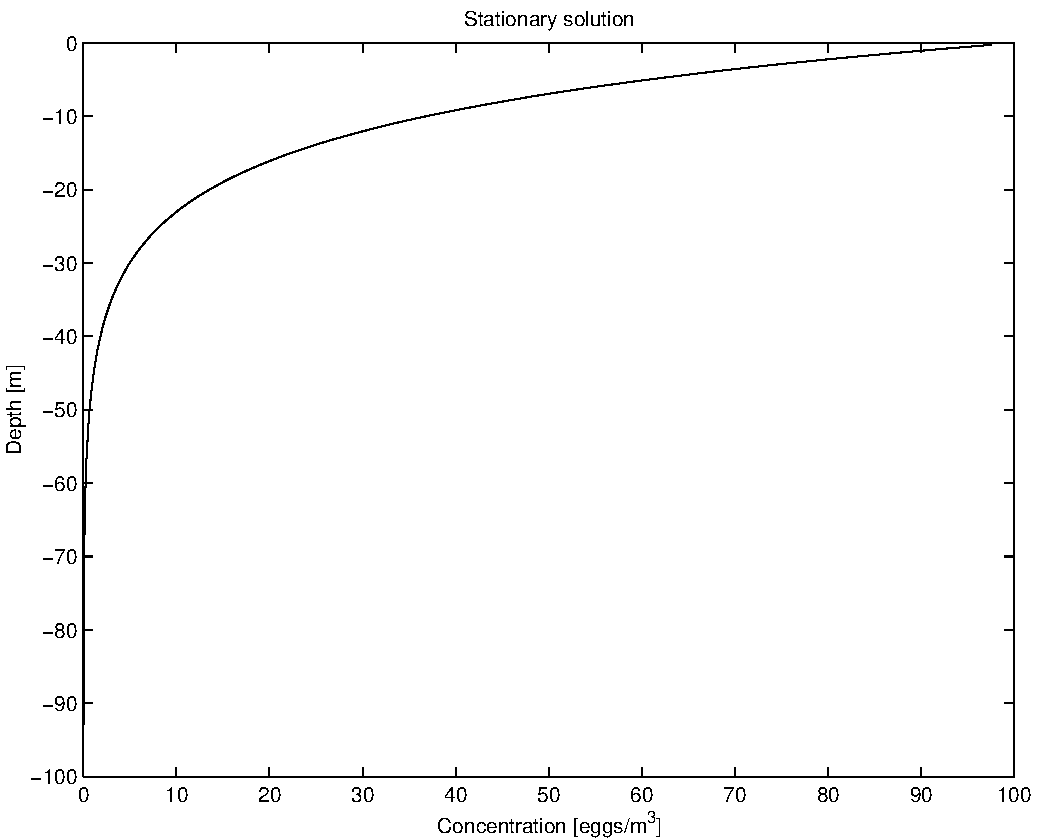
\includegraphics[height=8cm]{ex1a}
\end{center}
\caption{Steady state solution with constant coefficients and no 
         source terms}\label{fig:ex1a}
\end{figure}

The script \edb{srcsampl} demonstrates the exact solution
\edb{srcsact} with source terms. Using the same values of
\edb{K} and \edb{W} and spawning rate $1 \, \mbox{egg}/\mbox{m}^3/\mbox{day}$.
and mortality of 5\% per hour. The mortality rate \edb{alpha} is
computed by $exp(-\alpha \Delta t) = 1 - 0.05$.  The integrated steady
state concentration in this case is $\alpha / ( P * H) = 81.2
\,\mbox{eggs}/\mbox{m}^2$.

The solution is computed by the following code segment
\begin{verbatim}
  K = 0.01;  
  W = 0.001;
  P = 1/(24*3600);   
  alpha = -log(0.95) / 3600;
  A = srcsact(K,W,P,alpha);
\end{verbatim}

The steady state solution \edb{A} is depicted in figure~\ref{fig:ex1b}.
The main difference from the nosource situation is that
the concentration stays well above zero except very close to the
bottom, where no eggs come up from below.

\begin{figure}
\begin{center}
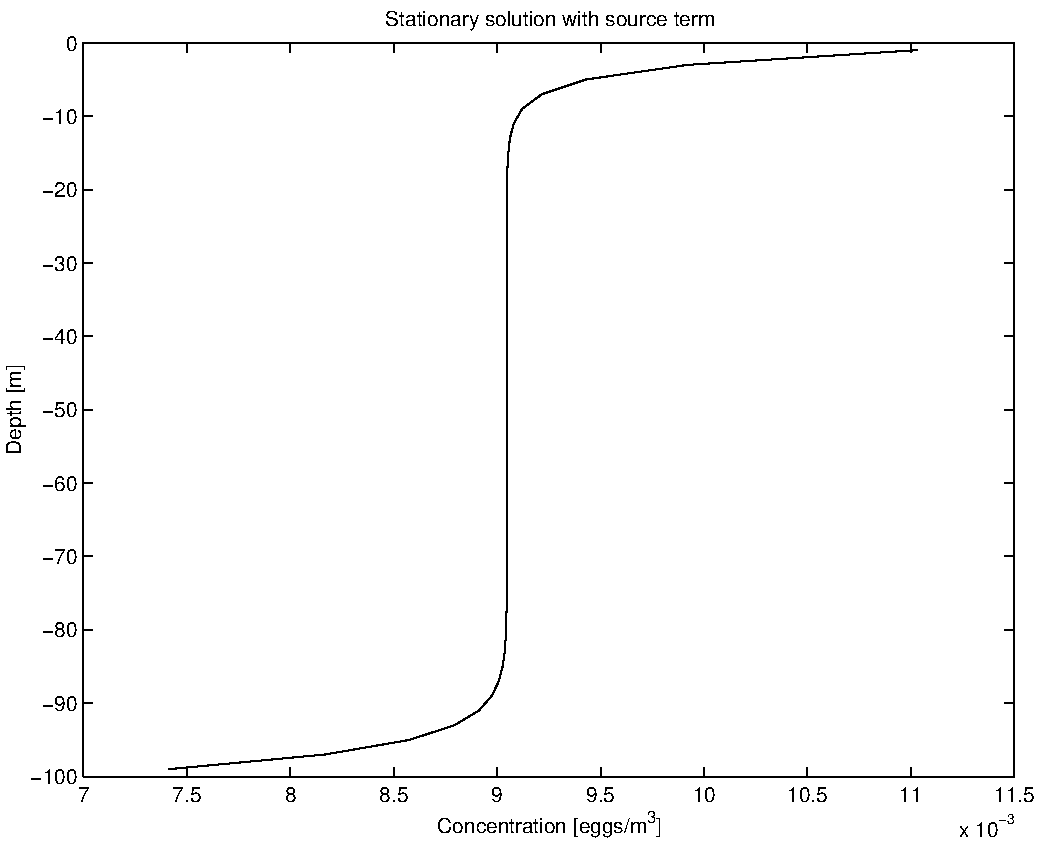
\includegraphics[height=8cm]{ex1b}
\end{center}
\caption{Steady state solution with constant coeffients including 
        spawning and mortality}\label{fig:ex1b}
\end{figure}

%\clearpage

\section{Example 2: Transient solution with constant coefficients}

This example demonstrates the use of \edbi{ftcs}, \edbi{lwendrof} or
\edbi{upstream} and \edbi{fluxlim} for solving the stationary problem
with constant values of eddy diffusivity and egg velocity. In addition
more visualisation techniques including animation is demonstrated.
The online scripts for this example is \edbi{runftcs}, \edbi{runus},
\edbi{runlw}, \edbi{runfl}, \edbi{plotex2} and \edbi{animex2}. Of these
one of the \edb{run}-scripts must be run first, to produce the data
for the visualization scripts.

The model is set up by giving values to the defining  parameters.

\begin{verbatim}
  H = 100;       % Depth [m] 
  dz0 = 2;       % Grid size [m]

  dt = 120;      % Time step [s]
  outstep = 1;   % Time between saving of model results [hours]
  simtime = 96;  % Total simulation time [hours] 
 
  K0 = 0.01;     % Eddy diffusivity [m^2/s]
  W0 = 0.001;    % Egg velocity     [m/s] 
 
  M0 = 1000;     % Vertical integral of concentration [eggs/m^2] 
\end{verbatim}

The space variables is used to initialize the grid for VertEgg.
\begin{verbatim}
  ve_init 
  ve_grid(H,dz0)
\end{verbatim}
Further time variables are needed
\begin{verbatim}
  nstep  = outstep*3600/dt; % Number of steps between outputs 
  nout   = simtime/outstep; % Number of output steps
\end{verbatim}
To make a start distribution concentrated at 50 m use the \edbi{spawn}
function
\begin{verbatim}
  A0 = spawn(M0, 50);
\end{verbatim}
alternatively a random initial condition can be given by 
\edb{A0 = ve\_rand(M0)}.\indextt{ve\_rand}

As the solvers need vectors as input, \edb{K0} and \edb{W0} must
be converted into constant column vectors.
\begin{verbatim}
  K = K0*ones(Ncell+1,1);
  W = W0*ones(Ncell+1,1); 
\end{verbatim}
We will use \edb{A} for the calculations and \edb{X} for saving
the results.
\begin{verbatim}
  A = A0;   
  X = [];   % Remove any old stuff in X 
\end{verbatim}
The time integration loop can be written as
\begin{verbatim}
  for t = 1:nout 
    A = lwendrof(A,K,W,nstep,dt); 
    X(:,t) = A; 
  end
\end{verbatim}

After computing the solution, the results must be analysed and
visualised. The final result from \edb{runlw} is stored in \edb{A}.
The following code-fragment plots
the profile of \edb{A} and the exact stationary solution \edb{B}.
\begin{verbatim}
  plot(A,ZE) 
  hold on   % Don't wipe out graphics before next plot
  B = eggsact(M0,K0,W0); 
  plot(B,ZE,'r') 
  hold off 
  legend('Numerical solution', 'Exact solution')
\end{verbatim}
For Octave remove the \edb{legend} statement.

The convergence of the solution to a steady state can be studied by
looking at the time development of the mean.
\begin{verbatim}
  T  = [1:nout];
  TL = T*outstep;         % Time labels 
  mu = ve_mean(X);        % The means 
  plot(TL,mu) 
\end{verbatim}
An alternative is to look at the root mean square deviation
from the exact solution \edb{B}.\indextt{ve\_rmsd}
(!!! Sjekk om her er noe semilog-greier )
\begin{verbatim}
  R = ve_rmsd(X,B);
  plot(TL,R)
\end{verbatim}
By removing the first 24 hours, the convergence is easier to see.
This result is depicted in figure~\ref{fig:ex2}
\begin{verbatim}
  T2  = [24:nout];
  TL2 = T2 * outstep;
  plot(TL2, R(T2));
\end{verbatim}
  
\begin{figure}
\begin{center}
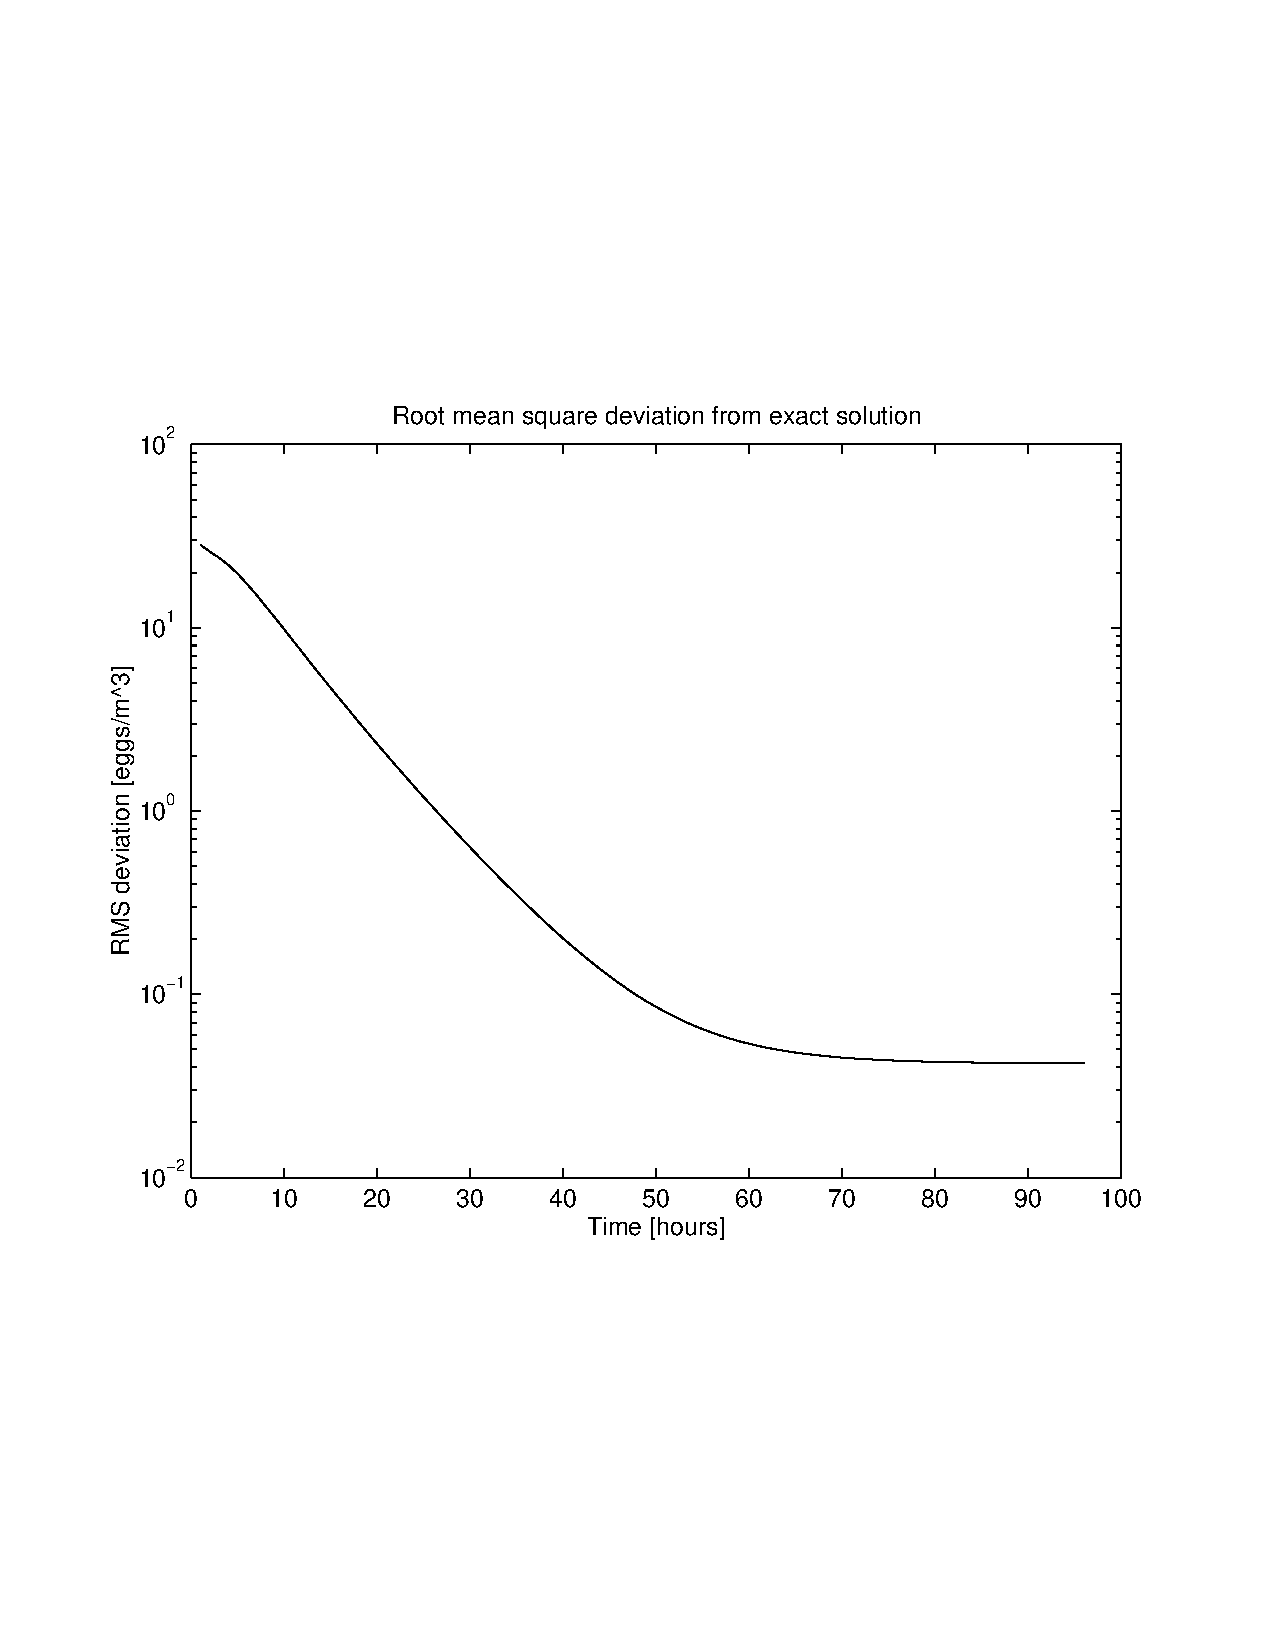
\includegraphics[height=8cm]{ex2}
\end{center}
\caption{Convergence to steady state with Lax-Wendroff method}\label{fig:ex2}
\end{figure}

The two next figures are MATLAB only. Surface graphics in
Octave/gnuplot is to primitive yet. The first is a isoplet
diagram, a contour plot of the solution in the time-depth plane.
\begin{verbatim}
  cl = [10:10:110];  % Contour levels 
  c = contour(TL,ZE,X,cl); 
  clabel(c) 
\end{verbatim}
A more spectacular view of the same surface in 3D.
\begin{verbatim}
  surf(TL,ZE,X); 
\end{verbatim}

The last script \edb{animex2} animates the time evolution of the
numerical solution. Under MATLAB be careful to make the graphic 
window visible and disjoint from the command window, otherwise
the command window will be raised and hide the animation.
The MATLAB animation code is simply.
\begin{verbatim}
  T = [1:nout]; 
  for t = T 
    title_string = sprintf('Time = %d', t*outstep) 
    plot(X(:,t),ZE) 
    title(title_string) 
    axis([0 120 -Hcol 0]) 
    drawnow 
  end
\end{verbatim}
The Octave code is nearly the same.
\begin{verbatim}
  T = [1:nout]; 
  axis([0 120 -Hcol 0]) 
  for t = T 
    title_string = sprintf('Time = %d', t*outstep); 
    title(title_string); 
    plot(X(:,t), ZE) 
  end
\end{verbatim}
If the animation is too fast, put the statement
\edb{pause(1)} somewhere in the loop.


\section{Example 3, Sensitivity studies}\label{sec:sens}

In this example, the performance of the different numerical schemes
from section~\ref{sec:numtrans} is tested. The testing is done by the
script \edbi{runsens}.  The testing is done by running the schemes
with constant coefficients until steady state and thereafter comparing
with the exact solution computed by \edbi{eggsact}. The parameters
that are varied are the eddy diffusion coefficient $K$, the vertical
velocity $w$, the space step \edb{dz} and the time step \edb{dt}.
These are defined near the start of the file \edb{runsens.m}.
\begin{verbatim}
  % Diffusion coefficient [m^2/s]
  K0 = 0.01;
  % Vertical velocity     [m/s]
  W0 = 0.001;         
  % Space step            [m]
  dz0 = 2;                
  % Time step             [s]
  dt = 120;  
\end{verbatim}
These values are the same as in example 2. 
The other defining variables are
\begin{verbatim}
  H = 100;       % Depth [m]
  simtime = 72;  % Simulation time [hours]
  M0 = 1000;     % Vertical integral of concentration [eggs/m^2]
\end{verbatim}
From example 2 it is evident that the result after 72 hours is close
to the steady state limit.
All eggs are released at depth 50 m.

After initialising VertEgg, the characteristic numbers are computed
\begin{verbatim}
  C     = W0 * dt/dz;
  S     = K0 * dt/(dz*dz);
  Pcell = abs(C)/S;
\end{verbatim}
they are printed nicely in the command window by the C-style output
function \edbi{fprintf}.

The number of timesteps is
\begin{verbatim}
  nstep  = simtime*3600/dt;  % Number of steps 
\end{verbatim}

Testing the first scheme is done by
\begin{verbatim}
  tic           % Reset clock
  A = ftcs(A0,K,W,nstep,dt);
  tid(1) = toc; % Save elapsed time 
  X(:,1) = A;   % Put solution as first column in X
\end{verbatim}
and similar for the other three methods. The timing was done
on a PC with an INTEL 486 processor running at 66 MHz.

The exact solution and some of it properties is computed by
\begin{verbatim}
  B = eggsact(M0,K0,W0);
  Bmean = ve_mean(B);
  Bstd  = ve_std(B);
\end{verbatim}
Thereafter the root mean square error, and the errors in mean depth
and standard deviation is computed by
\begin{verbatim}
  R = ve_rmsd(X,B);
  Emean = ve_mean(X) - Bmean;
  Estd  = ve_std(X) - Bstd;
\end{verbatim}
For plotting purposes, the errors in the methods are given 
as the columns in \edb{Y}.
\begin{verbatim}
  Y = X - B *ones(1,4);
\end{verbatim}
The results are summarized in a table, made by the \edb{fprintf}
command.  A better formatted version of this table for a standard run
is given in table~\ref{tab:ex3a}.

While performing such sensitivity tests under MATLAB the \edbi{diary}
function can be useful. It saves the commands and responces in the
text window to a file for later use.

The tests presented here belong to two groups. The first has
$K = 0.01 \sqmps$ and $W = 0.001 \mps$, the same values as used in
previous examples. The exact stationary solution with \edb{dz} = 1 is given
as fig~\ref{fig:ex1a}. 

The reference run is done by with a space step of 2\m and a time step
of two minutes. The resulting solutions are given in
fig.~\ref{fig:ex3a}. All methods, except the upstream scheme, produced
solutions that can not be distinguished from each other (and the exact
solution) in the figure. The upstream scheme gives a lower peak at the
surface and too high concentrations below 10 m. Figure~\ref{fig:ex3b}
plots the error, that is the diffence between the numerical solution
and the exact solution. As Lax-Wendroff is positive, the flux limited
method produce the same solution. The FTCS scheme slightly overshoots
the surface value, while Lax-Wendroff undershoots even more slightly.
The table for this run is table~\ref{tab:ex3a} below.

\begin{table}[h]
\begin{center}
\begin{tabular}{||l|r|r|r|r||}
\hline
    &  RMSE  & E-mean & E-std & CPU-time \\
\hline
ftcs     & 0.050 &  0.029 & -0.026 &  8.7  \\
lwendrof & 0.044 & -0.030 &  0.034 &  8.5  \\
upstream & 1.421 & -0.965 &  0.951 &  8.6  \\
fluxlim  & 0.044 & -0.030 &  0.034 & 11.8  \\
\hline
\end{tabular}
\end{center}
\caption{Results from reference run}\label{tab:ex3a}
\end{table}

\begin{figure}
\begin{center}
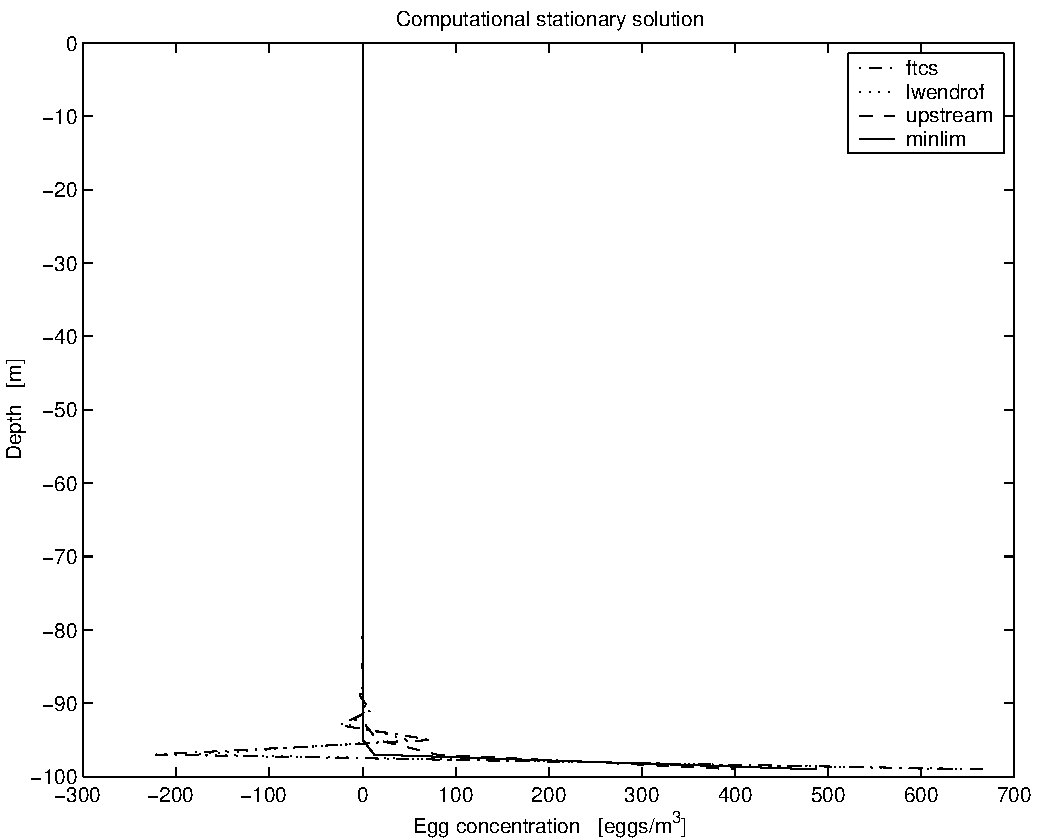
\includegraphics[height=8cm]{ex3a}
\end{center}
\caption{The numerical stationary solutions with parameters,
     $K = 0.01 \sqmps$, $w = 0.001 \mps$, $\edb{dz} = 2\m$, 
     $\edb{dt} = 120\s$}\label{fig:ex3a}
\end{figure}

\begin{figure}
\begin{center}
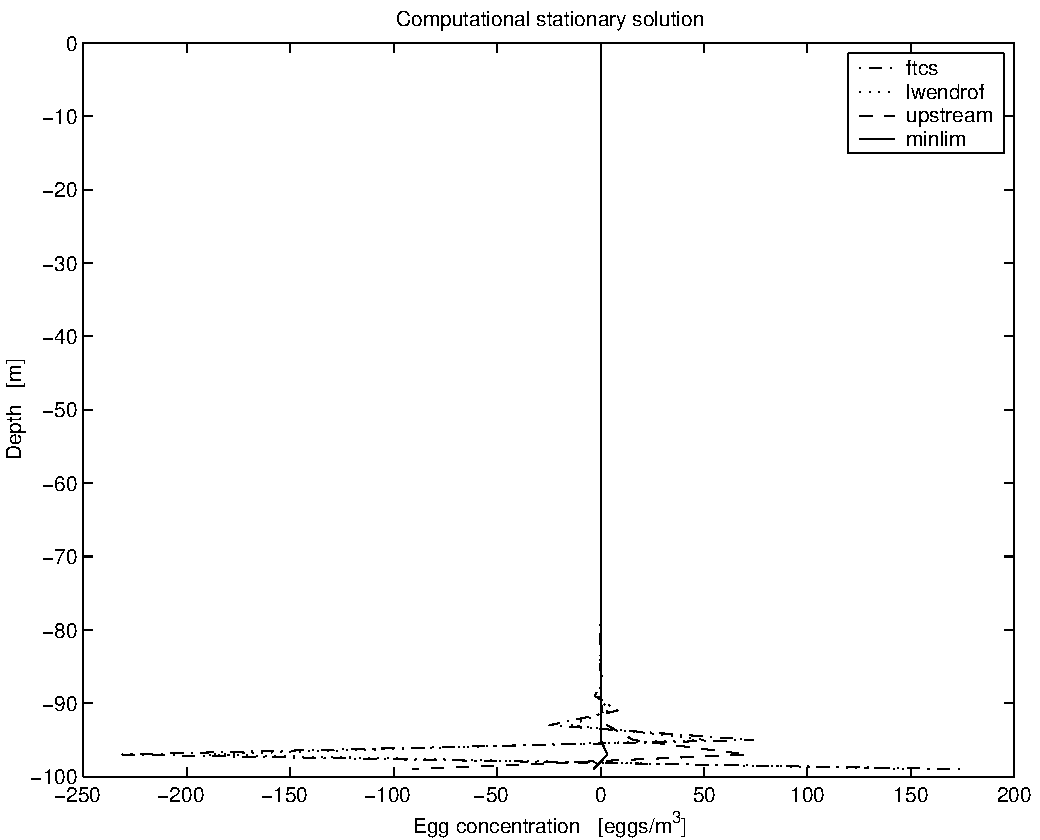
\includegraphics[height=8cm]{ex3b}
\end{center}
\caption{The errors in the numerical stationary
         solutions above}\label{fig:ex3b}
\end{figure}


The other class of tests is meant to be typical of sinking eggs.
Here the eddy diffusivity is 5 per cent of the above,
$K = 0.0005 \sqmps$ and $w = -0.001 \mps$. 
To plot the exact solution
for a subrange of the water column, an index array is used.
\begin{verbatim}
  B = eggsact(M0,K0,W0);
  II = 41:50;  
  plot(B(II),SE(II))
\end{verbatim}
This figure is given as figure~\ref{fig:ex3c}.

The corresponding numerical solutions ($\edb{dz} = 2 \m$, $\edb{dt} =
120 \s$) are shown in figure~\ref{fig:ex3d}. Both the FTCS and the
Lax-Wendroff scheme have produced oscillations and negative values.
The upstream solution is quite smeared out, while the flux limited
method seem to perform quite well. The table for this run is
tab~\ref{tab:ex3sinc}.


\begin{figure}
\begin{center}
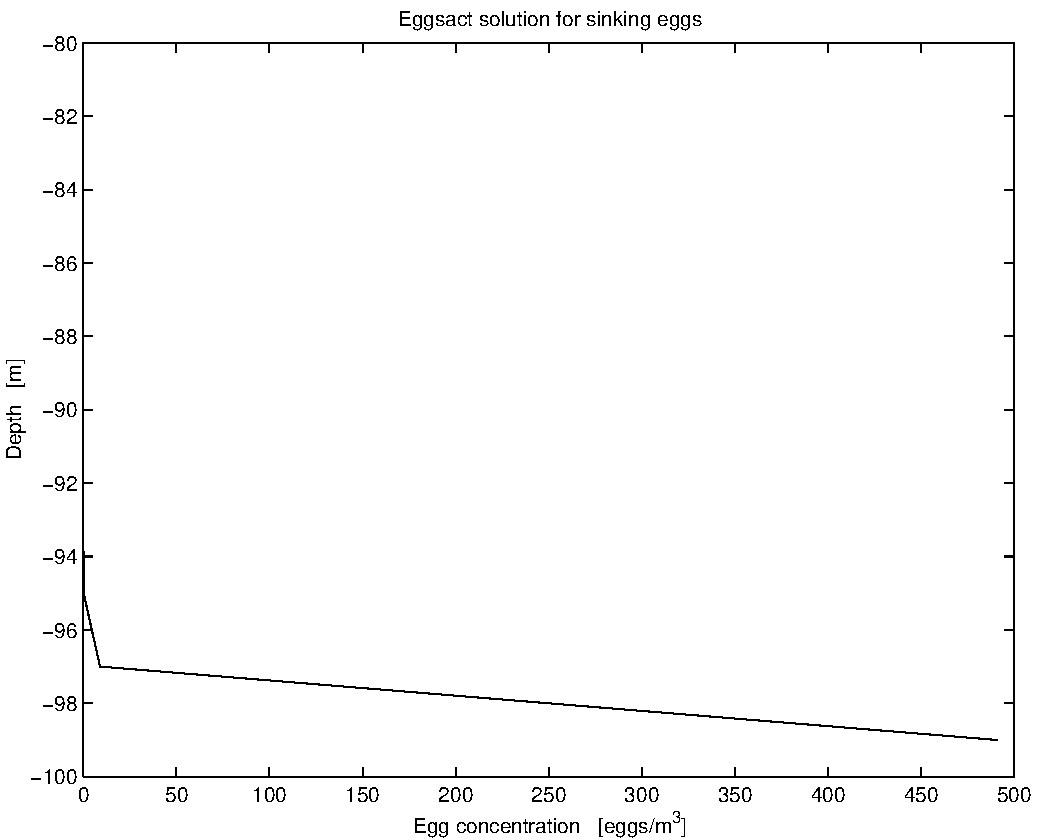
\includegraphics[height=8cm]{ex3c}
\end{center}
\caption{The exact stationary solution with%
     $K = 0.0005 \sqmps$, $w = -0.001 \mps$,%
     $\edb{dz} = 2 \m$}\label{fig:ex3c}
\end{figure}

\begin{table}[h]
\begin{center}
\begin{tabular}{||l|r|r|r|r||}
\hline
    &  RMSE  & E-mean & E-std & CPU-time \\
\hline
ftcs     & 42.549 & -0.537 & -0.640 &  8.6  \\
lwendrof & 35.038 & -0.477 & -0.640 &  8.5  \\
upstream & 16.466 & -0.463 &  0.618 &  8.6  \\
fluxlim  &  0.718 & -0.014 & -0.022 & 32.8  \\
\hline
\end{tabular}
\end{center}
\caption{Results from standard sinking run}\label{tab:ex3sinc}
\end{table}

\begin{figure}
\begin{center}
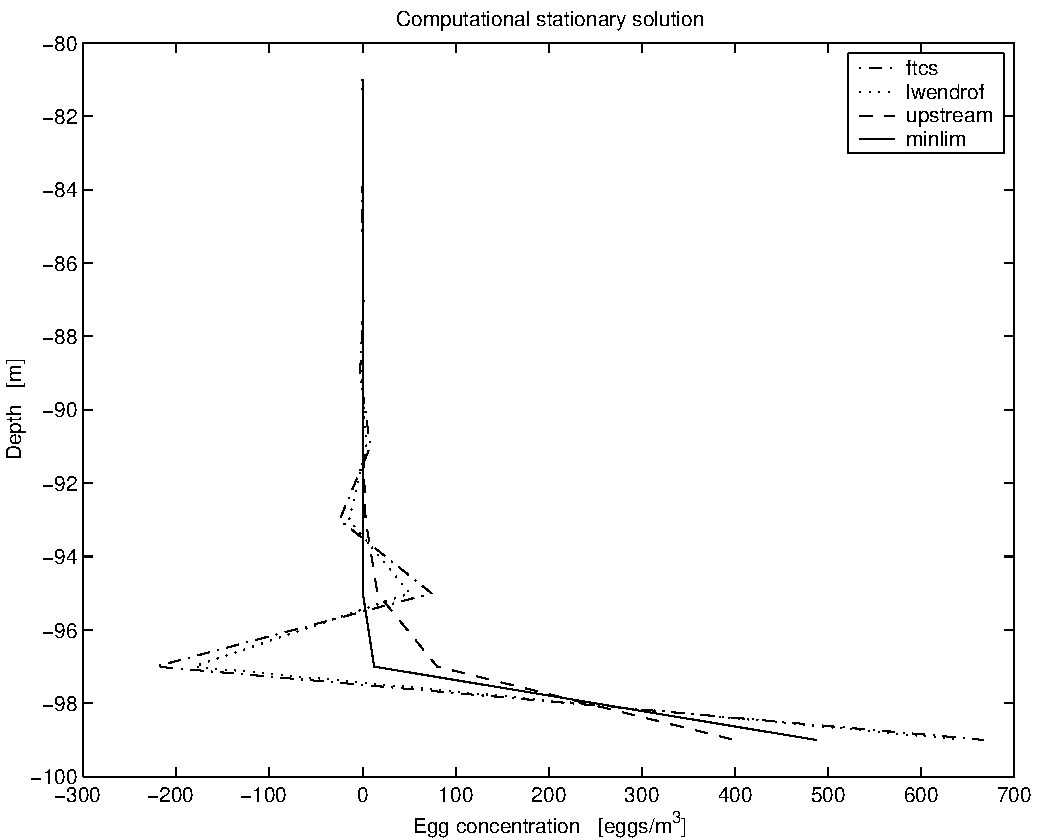
\includegraphics[height=8cm]{ex3d}
\end{center}
\caption{The numerical stationary solutions with parameters,
     $K = 0.0005 \sqmps$, $w = -0.001 \mps$, $\edb{dz} = 2 \m$, 
     $\edb{dt} = 120 \s$}\label{fig:ex3d}
\end{figure}


\clearpage

\section{Example 4, Terminal egg velocity}

This example verifies and demonstrates the function \edbi{eggvel} for
computing the terminal egg velocities.  The script is \edbi{velex} in
the example directory. Incluided in this example is also the script
\edb{visklsq} which performs the least squares regression used to
derive formula~\eqref{eq:molvisc} for the dynamic molecular viscosity.

First some necessary constant are defined,
\begin{verbatim}
  mu = 1.6e-3;         % Dynamic molecular viscosity 
  g = 9.81;            % Acceleration due to gravity 
  rho = 1027;          % Density of sea water
\end{verbatim}
%% Sjekk korrekt verdi for mu
then the maximum egg diameter \edb{Dmax} for application of
Stokes' formula can be plotted
\begin{verbatim}
  drho = [0.1:0.1:5];      % Range of density differences 
  Dmax = ( 9 * mu^2 ./ (rho * g * drho) ).^(1/3); 
  plot(drho, Dmax * 1000)  % Use mm as unit 
\end{verbatim}

As a verification of the implementation of the formulas in 
\edbi{eggvel}, figure~1 from Sundby \shortcite{sund83} will be
reproduced.
\begin{verbatim}
  d = [0:0.1:5];   % Range of diameters (in mm) 
  hold on 
  axis([0 5 0 5]); 
  for drho = [0.25 0.5 1:6]  % The values of drho used by Sundby 
    W = eggvel(drho * ones(size(d)), d/1000, mu); 
    plot(d, W*1000, 'g')
  end
\end{verbatim}
The expression \edb{drho*ones(size(d))} is required to make \edb{drho}
into an array of the same shape as \edb{d}, as required by
\edb{eggvel}. The factors 1000 converts between \mm\ and \m.
The lines $Re = 0.5$ and $Re = 5.0$ are added in red colour.
This figure is shown as fig.~\ref{fig:ex4a}.
\begin{verbatim}
  d(1) = [];          % Remove d(1) to prevent division by zero
  W = 0.5 * mu ./ (rho * d/1000); 
  W = 1000 * W;       % Convert to mm/s 
  hold on 
  plot(d, W, 'r');    % Re = 0.5 
  plot(d, 10*W, 'r'); % Re = 5.0 
  hold off 
\end{verbatim}


\begin{figure}
\begin{center}
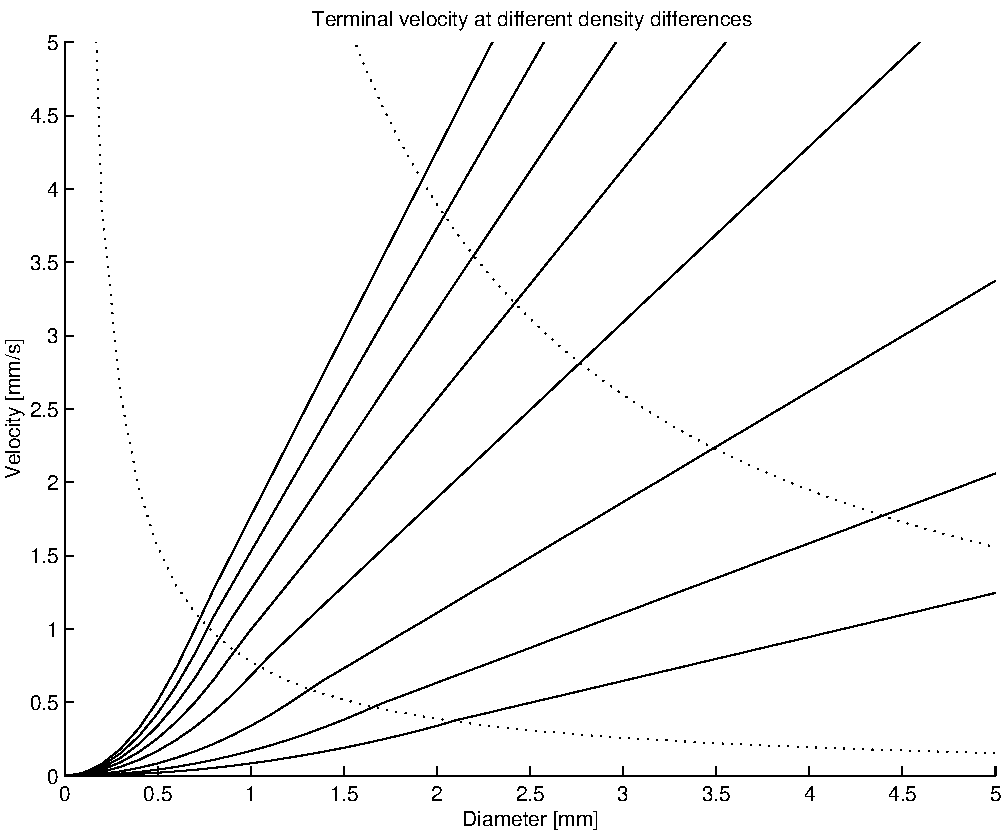
\includegraphics[height=8cm]{ex4a}
\end{center}
\caption{Terminal velocity for different density differences}\label{fig:ex4a}
\end{figure}


Another way of visualizing the \edbi{eggvel} function is to make a
table and make a contour plot of it. The rest of this example is for
MATLAB only.  Tables for \edb{W} and \edb{Re} are made by the
following commands,
\begin{verbatim}
  d = [0:0.1:4];      % mm 
  drho = [0:0.2:6];   % kg/m^3 
  dtab = ones(size(drho))' * d / 1000;  % d constant in colums 
  drhotab = drho' * ones(size(d));  % drho constant in rows  
  [W Re] = eggvel(drhotab, dtab); 
\end{verbatim}
The contour plot is made by.
\begin{verbatim}
  cl = [0.1:0.1:0.5 1.0:0.5:3.0 4.0:9.0]; % Contour levels 
  c = contour(d, drho, 1000*W, cl, 'g'); 
  clabel(c)
\end{verbatim}
Add the same lines $Re = 0.5$ and $Re = 5.0$ in red as above.
\begin{verbatim}
  hold on 
  cl = [0.5 5.0]; 
  contour(d, drho, Re, cl, 'r'); 
  hold off
\end{verbatim}
A 3D view of the velocity surface can also be plotted.
\begin{verbatim}
  surf(d, drho, 1000*W) 
\end{verbatim}

\begin{figure}
\begin{center}
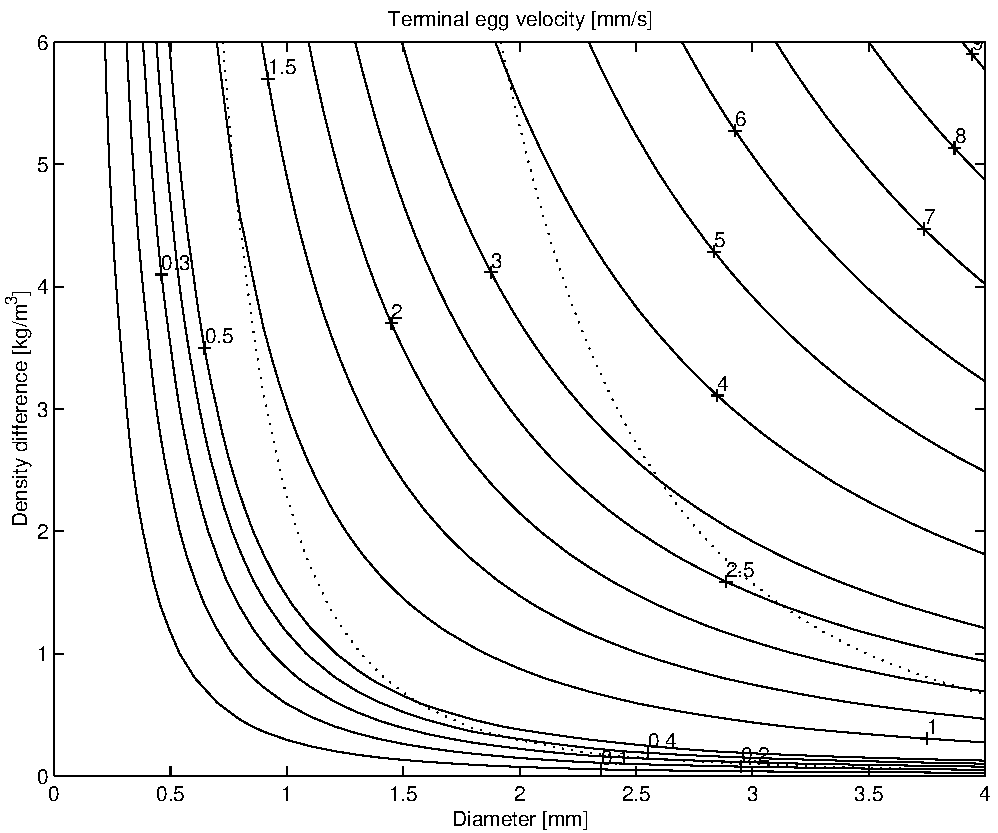
\includegraphics[height=8cm]{ex4b}
\end{center}
\caption{Terminal velocity contours}\label{fig:ex4b}
\end{figure}


Systems like MATLAB and Octave are well suited for fitting functions
to data. The script \edbi{visklsq} demonstrates how to fit a
polynomial, quadratic in $T$ and linear in $S$ to
table~\ref{tab:molvisc} by the method of least squares\index{least
squares}.  Some array manipulation must first be done to obtain
three column vectors \edb{SI}, \edb{TI} and \edb{B} with corresponding
values of salinity, temperature and viscosity. With $\edb{MN} = 35 = 5
\times 7$, the normal matrix is simply
\begin{verbatim}
  A = [ones(MN) TI  TI.^2 SI];  
\end{verbatim}
In MATLAB the vector \edb{X} of coefficients is found by
\begin{verbatim}
  V = eye(MN);       % Covariance matrix = identity 
  X = lscov(A,B,V);  
\end{verbatim}
in Octave the same task is done by
\begin{verbatim}
  X = ols(B,A);
\end{verbatim}


\section{Example 5, Non-constant coefficients}

This example illustrates how to use several egg groups on a transient
problem with non-constant coefficients. It also provides a verification of
parts of the toolbox by reproducing results by Westg{\aa}rd \shortcite{west89}.
The model is contained in the script \edbi{runex5}. The results are
visualized by the scripts \edbi{plotex5} and by animation in
\edbi{animex5}.

The problem is the first example from \cite{west89}. The bottom depth
is 100\m\ and a grid size of 2\m\ is used.
\begin{verbatim}
  ve_init
  ve_grid(100,2)
\end{verbatim}
There is a pycnocline at 50\m, with temperature 7\degC\ and salinity 34
above and temperature 5\degC\ and salinity 35 below.
\begin{verbatim}
  I25 = ones(25,1);        
  S(1:25) = 34*I25; S(26) = 34.5; S(27:51) = 35*I25;
  T(1:25) =  7*I25; T(26) =  6  ; T(27:51) =  5*I25;
\end{verbatim}
The wind speed is 5\mps. The turbulent eddy viscosity in the upper
layer is computed by a formula form Sundby \shortcite{sund83}. The
turbulence in the lower layer is $1/10$ of the value in the upper
layer.
\begin{verbatim}
  Wind = 5;
  K0 = (76.1 + 2.26*Wind^2) * 1e-4;
  K(1:25) = K0*I25; K(26) = 0.55*K0; K(27:51) = 0.1*K0*I25;
\end{verbatim}
There are two groups of eggs, one with a diameter of 1.5\mm\ and
neutral buoyancy corresponding to 33 psu, and the other with a
diameter of 1.3\mm\ and neutral salinity 36 psu. The tool
\edbi{eggvelst} is used to compute the velocity profiles.
\begin{verbatim}
  d1  = 0.0015;
  Se1 = 33;
  W1  = eggvelst(S, T, d1, Se1); 
  d2  = 0.0013;
  Se2 = 36;
  W2  = eggvelst(S, T, d2, Se2); 
\end{verbatim}

The number of eggs are 55 in each group and the initial distribution
is the same step function in each group. The arrays \edb{A1} and
\edb{A2} are used for the concentrations within the groups.
\begin{verbatim}
  I10 = ones(10,1);
  A1( 1:10) = 0*I10;
  A1(11:20) = 0.75*I10;
  A1(21:30) = 1.25*I10;
  A1(31:40) = 0.75*I10;
  A1(41:50) = 0*I10;
  % Use the same initital distribution for group 2
  A2 = A1;
  % Save the intial distributions for later use.
  A10 = A1; A20 = A2;
  A0 = A10 + A20;
\end{verbatim}

The model is here run by the Lax-Wendroff scheme with a time step of 120\s\
and saving the result every 2nd hour. The total simulation time is 96
hours. 
\begin{verbatim}
  for t = 1:nout
    A1 = lwendrof(A1,K,W1,nstep,dt);
    X1(:,t) = A1;
    A2 = lwendrof(A2,K,W2,nstep,dt);
    X2(:,t) = A2;
  end
\end{verbatim}
Finally the results from the two groups are added,
\begin{verbatim}
  X = X1 + X2;
\end{verbatim}

\begin{figure}
\begin{center}
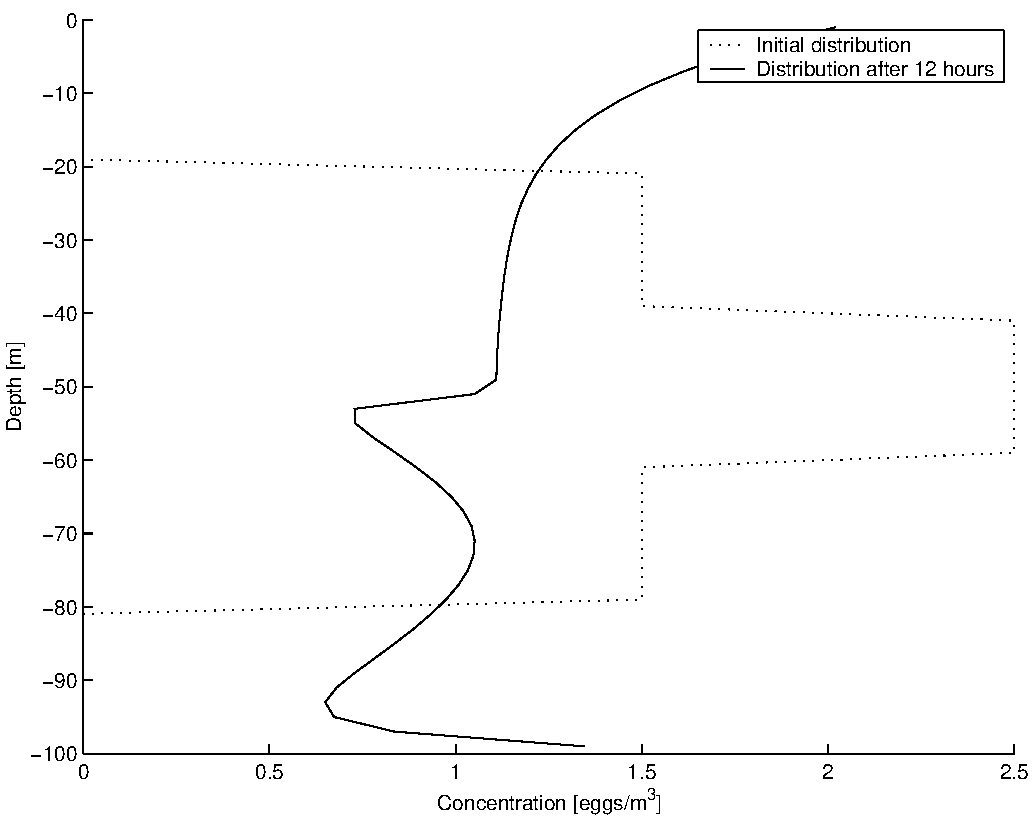
\includegraphics[height=8cm]{ex5a}
\end{center}
\caption{Figure 1 from Westg{\aa}rd (1989)}\label{fig:ex5a}
\end{figure}


Visualising the results with \edb{plotex5} the first task is to
reproduce figure 1 from Westg{\aa}rd \shortcite{west89}.
\begin{verbatim}
  t12 = 12 / outstep;
  hold on;
  plot(A0, ZE, 'y');        % The start distribution   
  plot(X(:,t12), ZE, 'g');  % After 12 hours
\end{verbatim}
This result is depicted in Fig.~\ref{fig:ex5a}.


With non-constant coefficients the function \edbi{sstate} must be used
to calculate the stationary solution.
\begin{verbatim}
  Y1 = sstate(M1,K,W1);
  Y2 = sstate(M2,K,W2);
  Y = Y1 + Y2;
\end{verbatim}
Adding this to the previous figure, gives Fig.~\ref{fig:ex5b}.
\begin{verbatim}
  plot(Y, ZE, 'r'); 
\end{verbatim}

\begin{figure}[h]
\begin{center}
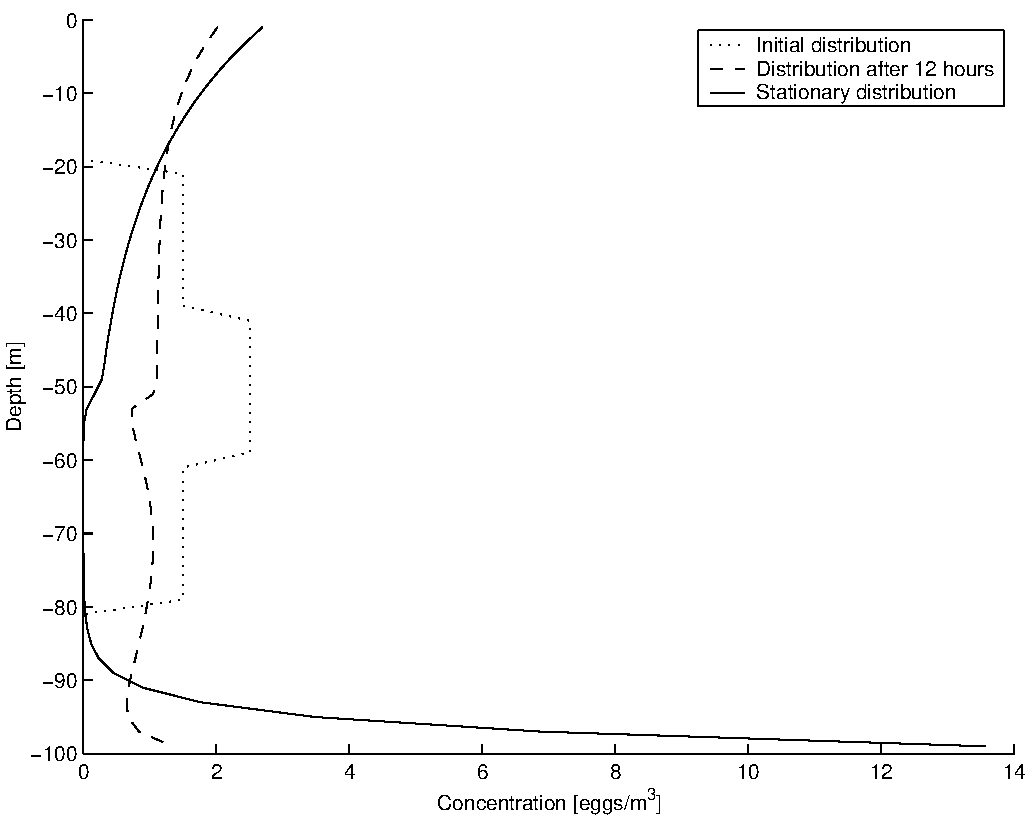
\includegraphics[height=8cm]{ex5b}
\end{center}
\caption{Initial, 12 hour and stationary limit solution}\label{fig:ex5b}
\end{figure}

In addition \edb{plotex5} and \edb{animex5} show more details on the
time evolution. For this example the steady state solution is reached
after approximately 80 hours.



\section{Example 6, Halibut eggs, the transient problem}

 
In this and the next two examples, eggs of Atlantic halibut
\emph{(Hippoglossus hippoglossus)} will be considered
in deeps fjords in northern Norway. Data on egg diameter and egg
salinity are taken from \citep{haug84}.  Synthetic vertical profiles,
representative for the area, of temperature, salinity and vertical
mixing have been constructed by S.~Sundby (pers.~comm.).

This example goes further towards developing a model application from
VertEgg. The main script \edbi{runex6} is initiated from the set-up file
\edb{runex6.sup}. The physical setting and initial egg distribution are
also read from files.
The model script is meant to be a prototype simulation model.
It should be easy to modify for similar simulations.
The script \edbi{plotini} is
used to plot the  physical and numerical situation before the
simulation, while \edbi{plotgrp3} and \edbi{plotres} are used for 
postprocessing of the model results. 

First the physical profiles will be plotted. 
The profiles are read from file and thereafter interpolated to
the flux points. The variable names are \edb{S} for salinty,
\edb{T} for temperature and \edb{K} for vertical mixing coefficient.
Several profiles are
combined into one figure by the Matlab command \edbi{subplot}.
\begin{verbatim}
  subplot(1,3,1)
  plot(S,ZF)
  title('Salinity')
  subplot(1,3,2)
  plot(T,ZF)
  title('Temperature')
  subplot(1,3,3)
  semilogx(K,ZF)   % Logarithmic X-axis
  title('Vertical mixing')
\end{verbatim}
The result is shown in fig.~\ref{fig:ex6a}

\begin{figure}[!htb]
\begin{center}
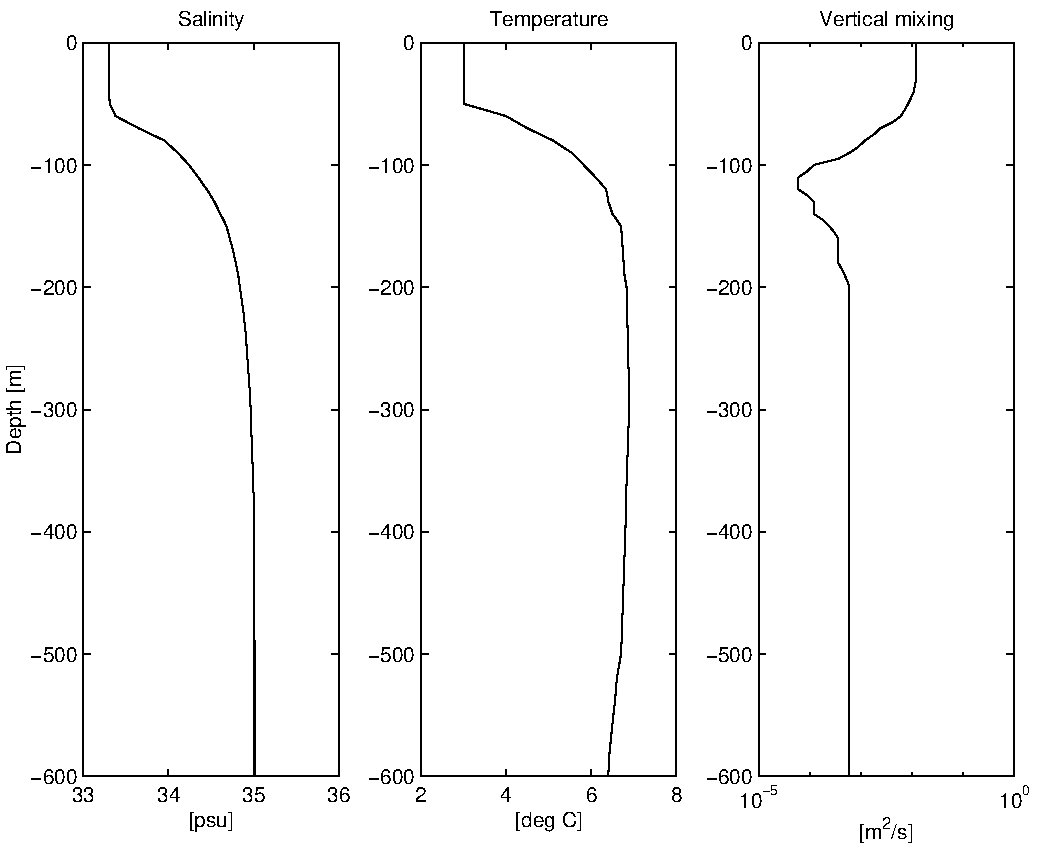
\includegraphics[height=8cm]{ex6a}
\end{center}
\caption{Vertical profiles of salinty, temperature and 
         vertical eddy viscosity}
\label{fig:ex6a}
\end{figure}

With the values 34.5 psu for egg salinity and egg diameter 3.2\mm,
\edbi{eggvelst} can be used to compute the egg velocity. Thereafter
the stationary solution with integrated density 100 eggs/m$^3$ can be
computed by \edbi{sstate}.
\begin{verbatim}
  eggsal = 34.5;
  eggdiam = 3.2;
  W = eggvelst(S,T,eggdiam/1000.0,eggsal);
  M = 100;
  ASS = sstate(M,K,W);
\end{verbatim}
The profiles are plotted in figure~\ref{fig:ex6b}. The vertical dotted
line in the left indicate zero velocity. 

\begin{figure}[!htb]
\begin{center}
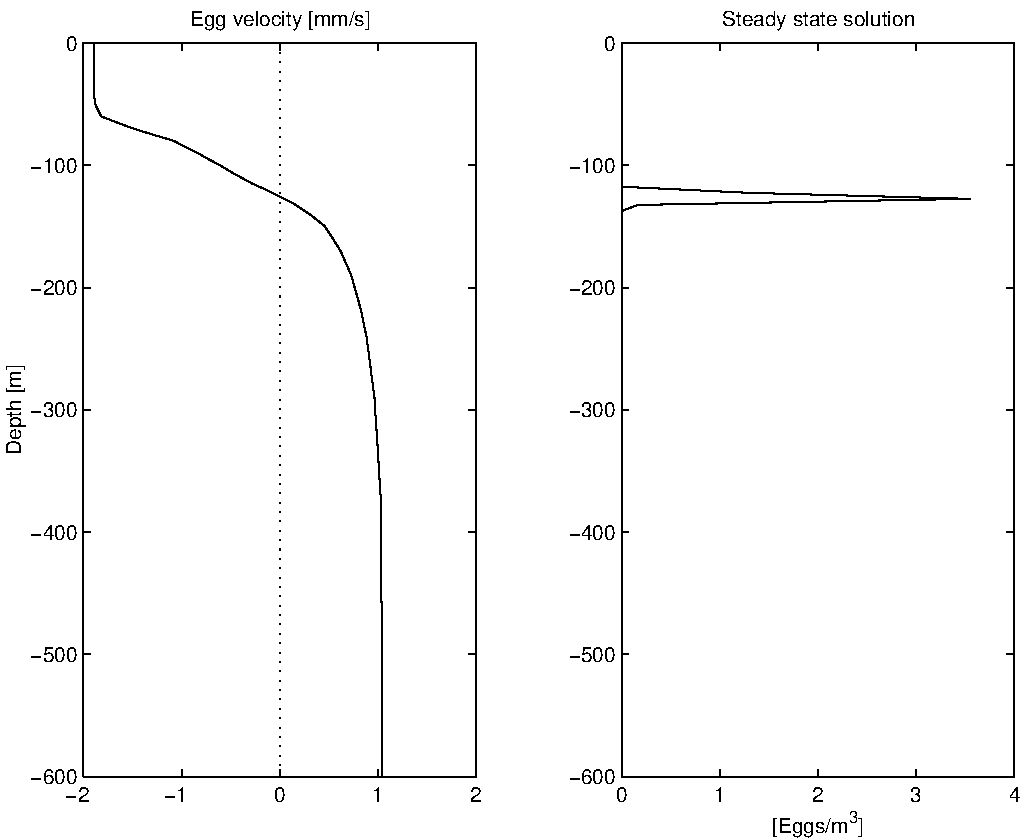
\includegraphics[height=8cm]{ex6b}
\end{center}
\caption{Egg velocity and stationary ditribution}
\label{fig:ex6b}
\end{figure}

The neutral salinity 34.5 occur at approximately 125\m\ depth, in the
pycnocline layer where the vertikal mixing coefficient is very
low. The stationary solution is therefore a very narrow peak at this
depth level.

Before running the transient simulation it is useful to look at the
numerical characteristics of the problem.  With $\Delta z = 5\m$ and
$\Delta t = 600\s$ the profiles are plotted in
figure~\ref{fig:ex6c}. 
All the three linear methods are stable.
However, the methods are not suitable because the high Peclet
numbers give high numerical diffusion in the upstream method and
produce negative values with FTCS and Lax-Wendroff. Therefore the more
time-consuming method \edbi{posmet} is used for the transient
simulations.


\begin{figure}[!htb]
\begin{center}
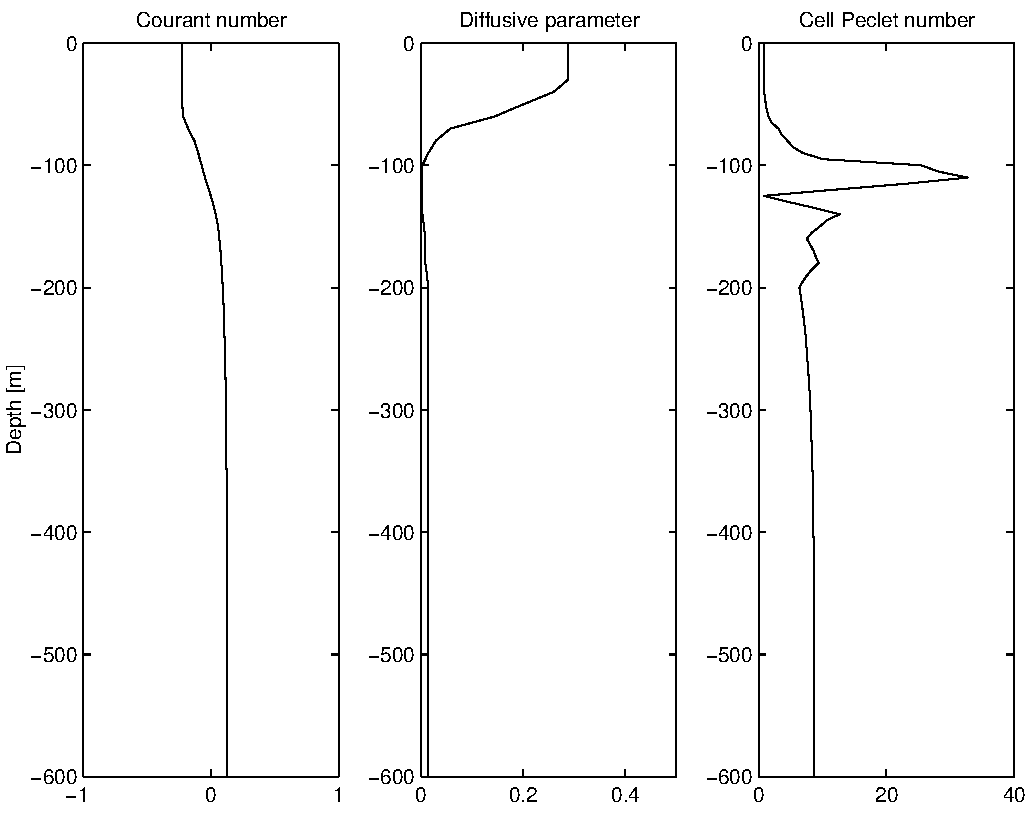
\includegraphics[height=8cm]{ex6c}
\end{center}
\caption{Vertical profiles of Courant number, diffusive parameter 
         and cell Peclet number}
\label{fig:ex6c}
\end{figure}

The model script start by reading the setup-file. Thereafter the
vertical physical profiles are read in and interpolated as above.
Similarly the inital egg distribution is read from file
\edb{halibut.dat} and interpolated to the egg points. 

Initially the eggs are distributed between 500 and 600\m\ depth.
The model is run with space step $\Delta z = 5\m$ and time
step $\Delta t = 10\, \text{minutes}$ as above. 5 egg groups are used,
all with diameter 3.2\mm\ but the neutral salinity vary from 34.3 to
34.7 psu in steps of 0.1. The simulation time is 10 days, and the
results are written to file every 12 hours.

The first post-processing script \edb{plotgrp3} concentrates on egg
group 3, which is neutral at salinity 34.5 psu.  The model output file
\edb{result.dat} is read and the egg profile data every 24 hour
starting with the initial distribution is 
stored in the array \edb{X3}. The command
\begin{verbatim}
  plot(X3,ZE)
\end{verbatim}
plots these daily distributions in fig.~\ref{fig:ex6d}. The numerics
seems to be working, the distributions do not contain negative values
and the eggs are moving upwards a little less then 100\m\ per day
without too much smoothing of the distribution. After 5--6 days the
distribution has reached it equilibrium level and start to concentrate
at this level. After the 10 days, the transient solution is very
similar to the stationary solutions. These solutions are compared in
figure~\ref{fig:ex6e}. The transient solution have a slightly higher
peak consentration.

\begin{figure}[!htb]
\begin{center}

\includegraphics[height=8cm]{ex6d}
\end{center}
\caption{Daily egg distributions from egg group 3}
\label{fig:ex6d}
\end{figure}

\begin{figure}[!htb]
\begin{center}
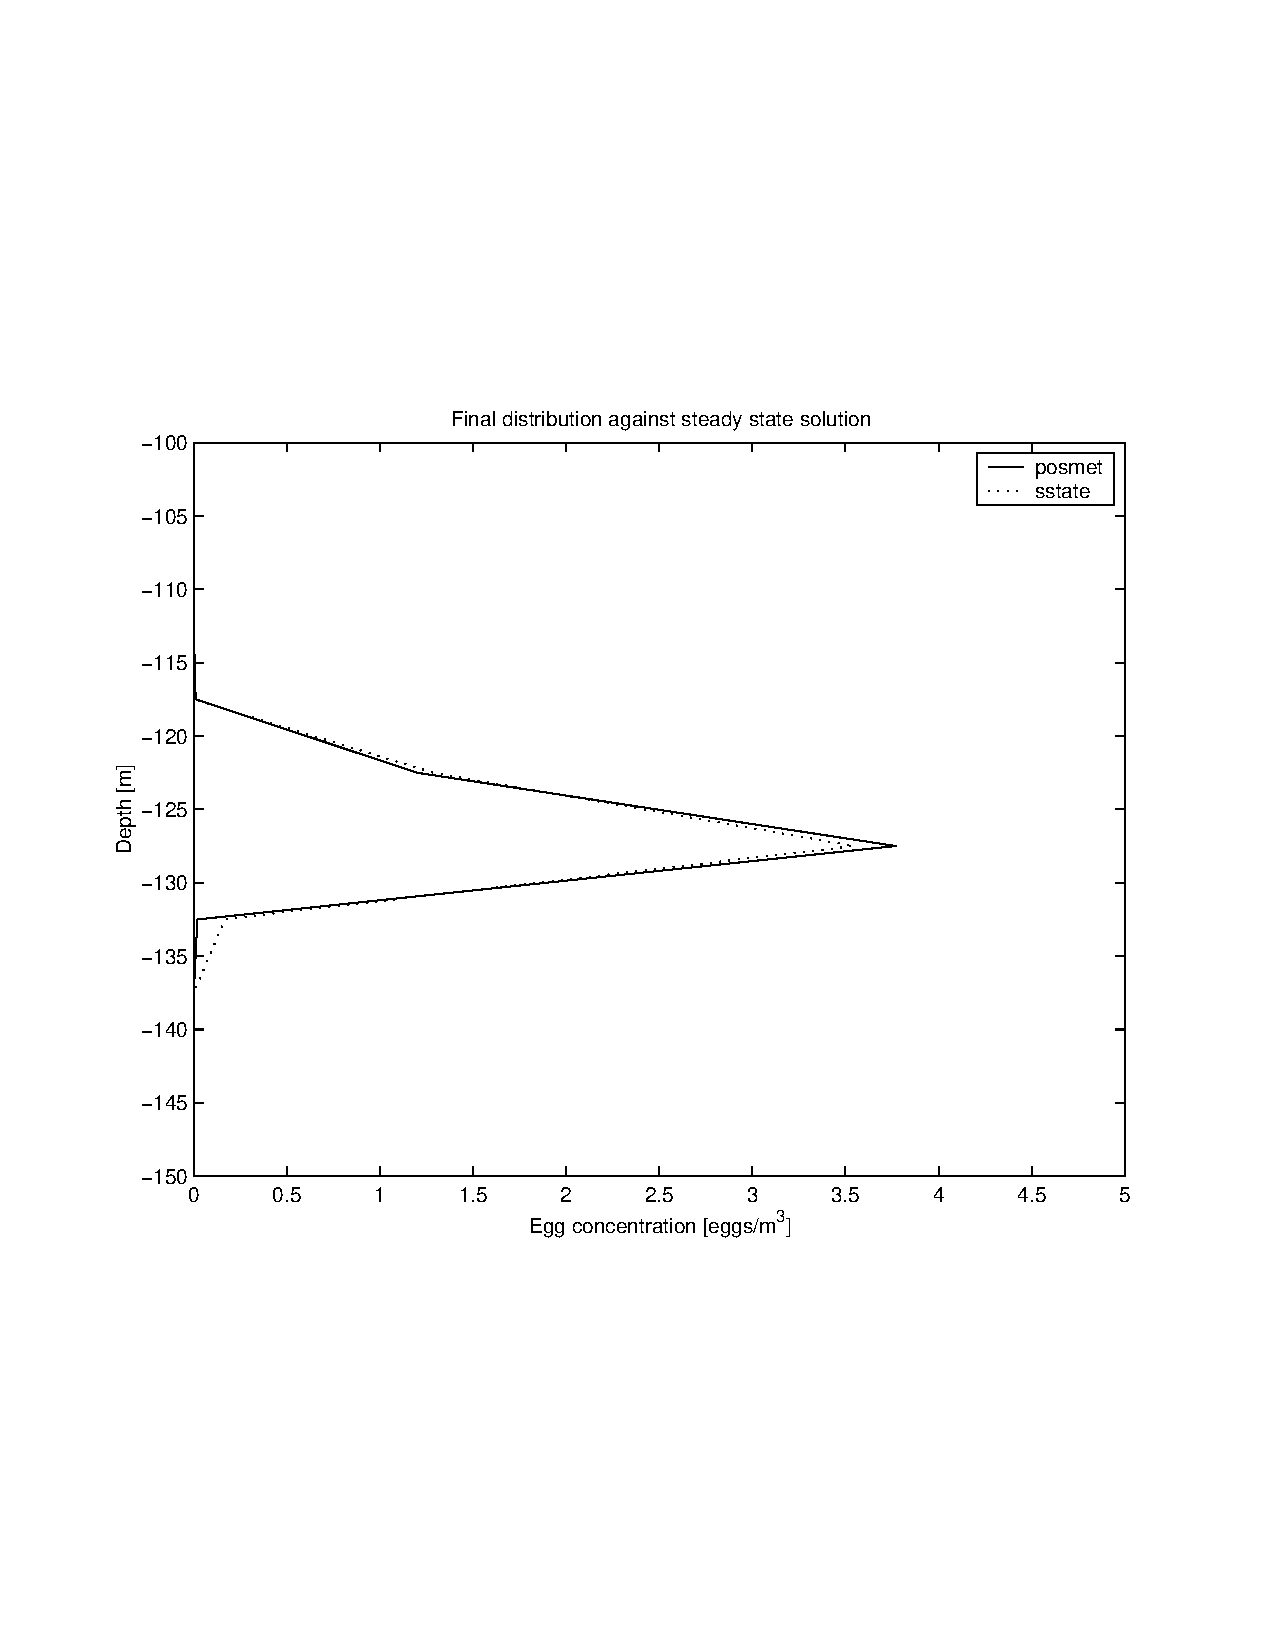
\includegraphics[height=8cm]{ex6e}
\end{center}
\caption{The distribution after 10 days compared to the
         steady state distribution from \edb{sstate}}
\label{fig:ex6e}
\end{figure}


The script \edbi{plotres} is used for postprocessing the results for
all 5 egg groups. In this case the columns in \edb{X} hold the sum of the
5 concentrations every 12 hour.
Figure~\ref{fig:ex6f} show the distributions for the 5 egg groups
after the 10 days of simulation. 
The solution is a narrow peak for each egg group at their equilibrium
salinity.


\begin{figure}[!htb]
\begin{center}
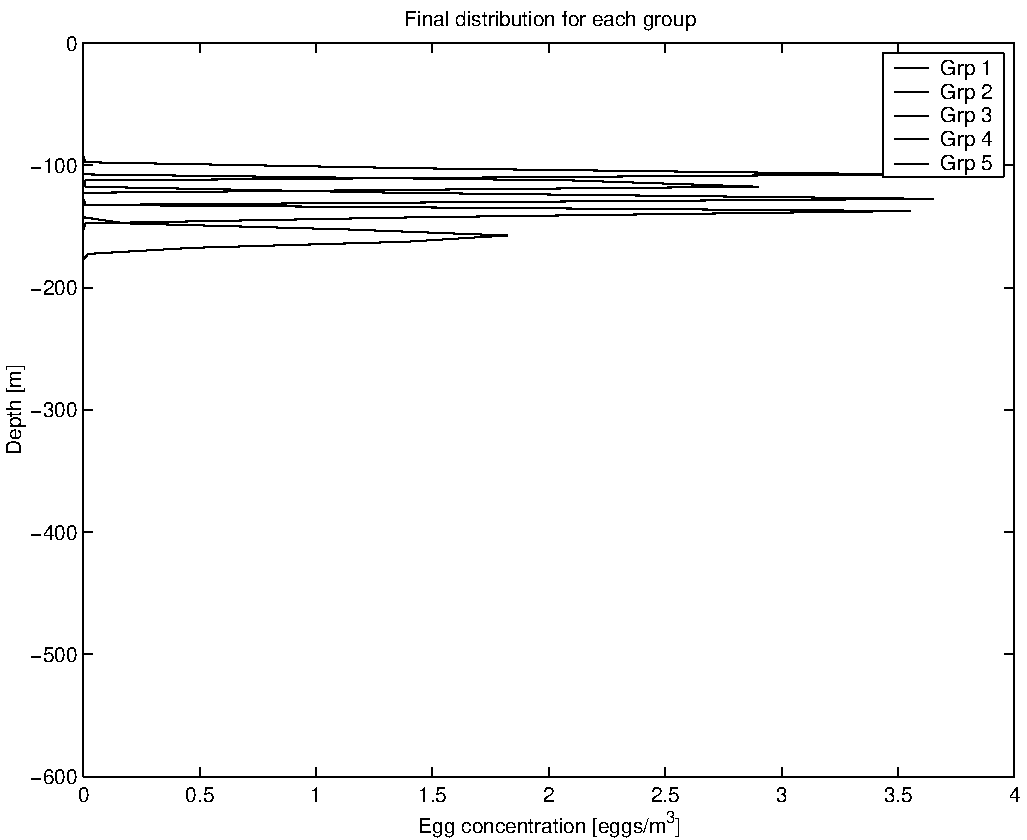
\includegraphics[height=8cm]{ex6f}
\end{center}
\caption{Final distribution of the 5 egg groups}
\label{fig:ex6f}
\end{figure}

The next figure~\ref{fig:ex6g} show the time evolution of the mean
depth of the distributions. Note that although the distance is shorter
the heaviest eggs use longer time to raise to their equilibrium
depth. This confirms unpublished calculations by S.~Sundby.

\begin{figure}[!htb]
\begin{center}
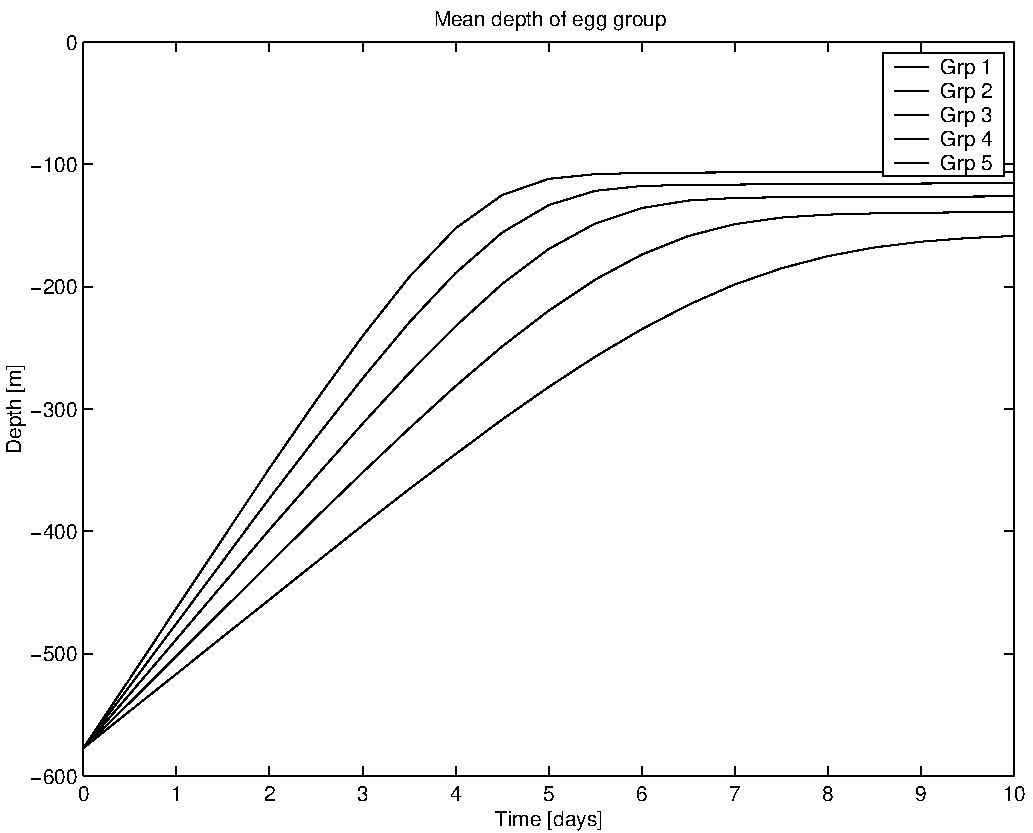
\includegraphics[height=8cm]{ex6g}
\end{center}
\caption{Time evolution of mean depth}
\label{fig:ex6g}
\end{figure}



\section{Example 7, Halibut eggs, Monte Carlo simulation}
\index{Monte Carlo}
{\bfseries Under construction}

In nature, egg diameters and densities are not constant or confined to
a handful of discrete groups. To explore this further it is assumed
that these properties have known statistical distributions.  The paper
\citep{haug84} does not identify the distributions but give ranges for
the values.  For the egg diameter a normal distribution with mean
3.2\mm\ and standard deviation 0.2\mm is used below. For the neutral
salinity of the egg a normal distribution with mean 34.5 psu and
standard deviation 0.2 psu is used. For simplicity it is assumed here
that egg diameter and egg salinity are independent.

In the script \edbi{runex7} a total of \edb{Nprof} egg diameters and 
corresponding egg salinities are
drawn randomly from the distributions above. Thereafter
\edbi{eggvelst} is used to compute the velocity profiles and
\edbi{sstate} computes the vertical distribution. The variable
\edb{Anorm} contains the average of the distributions so far,
normalised so that the vertical integral equal \edb{M} eggs/m$^2$.

The script \edbi{plotex7} is used to plot the results.
With \edb{Nprof} = 1000 the averaged vertical profile is given
in figure~\ref{fig:ex7a}. Nearly all the eggs are found 
between 50 and 300\m\ depth with high concentrations between 
100 and 200\m. Also note the few heavy eggs are  near bottom.

\begin{figure}[!htb]
\begin{center}
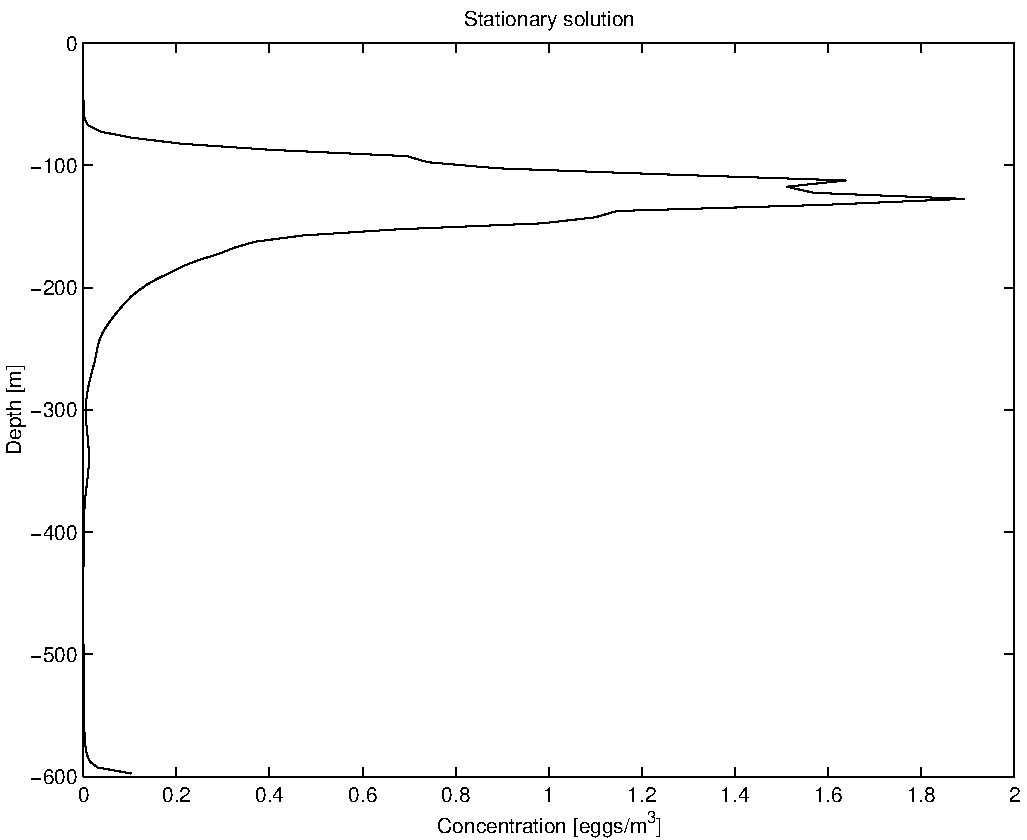
\includegraphics[height=8cm]{ex7a}
\end{center}
\caption{Vertical distribution of eggs from Monte Carlo run}
\label{fig:ex7a}
\end{figure}

Thereafter some statistics of this solution
is computed. Because of the randomness in the Monte Carlo process
these numbers (and the shape of fig.~\ref{fig:ex7a}) may vary from run
to run. In our case we obtain the following numbers. The egg diameters vary
from 2.57 to 3.85\mm\ with mean 3.19\mm\ and standard deviation
0.21\mm. The egg salinities vary from 33.87 to 35.22  with mean
34.50 and standard deviation 0.20 psu. The mean depth of the
distribution is 135.1\m and the standard deviation is 50.7\m.

To visualize the convergence of the Monte Carlo run, the root mean
square deviation of the normalised distribution after $i-1$ and $i$
iterations are saved in the array $R(i)$. Figure~\ref{fig:ex7b}
show the evolution of $R$ on a logarithmic scale. The convergence is 
quite slow, and 1000 samples may be too few. This explains why the
shape of the distribution may vary from run to run.

\begin{figure}[!htb]
\begin{center}
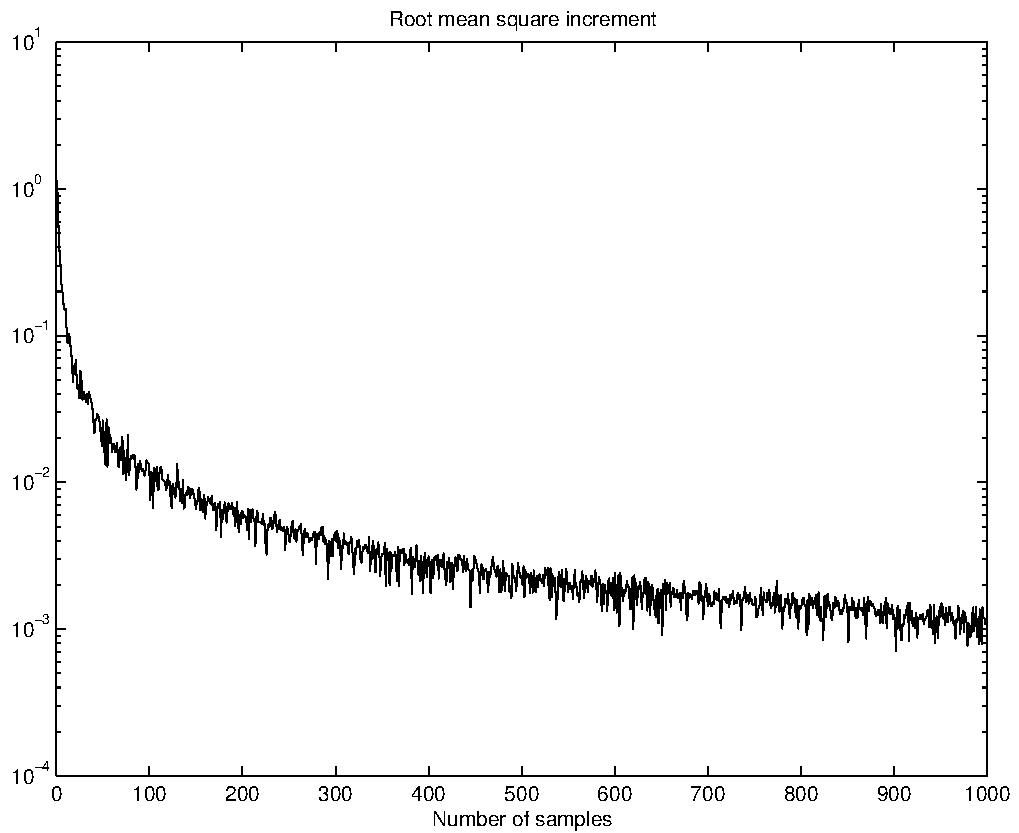
\includegraphics[height=8cm]{ex7b}
\end{center}
\caption{Development of the root mean square increment}
\label{fig:ex7b}
\end{figure}

\section{Example 8, Halibut eggs with spawning and hatching terms}
{\bfseries Under construction}


